\documentclass{ximera}

 

\usepackage{epsfig}

\graphicspath{
  {./}
  {figures/}
}

\usepackage{morewrites}
\makeatletter
\newcommand\subfile[1]{%
\renewcommand{\input}[1]{}%
\begingroup\skip@preamble\otherinput{#1}\endgroup\par\vspace{\topsep}
\let\input\otherinput}
\makeatother

\newcommand{\includeexercises}{\directlua{dofile("/home/jim/linearAlgebra/laode/exercises.lua")}}

%\newcounter{ccounter}
%\setcounter{ccounter}{1}
%\newcommand{\Chapter}[1]{\setcounter{chapter}{\arabic{ccounter}}\chapter{#1}\addtocounter{ccounter}{1}}

%\newcommand{\section}[1]{\section{#1}\setcounter{thm}{0}\setcounter{equation}{0}}

%\renewcommand{\theequation}{\arabic{chapter}.\arabic{section}.\arabic{equation}}
%\renewcommand{\thefigure}{\arabic{chapter}.\arabic{figure}}
%\renewcommand{\thetable}{\arabic{chapter}.\arabic{table}}

%\newcommand{\Sec}[2]{\section{#1}\markright{\arabic{ccounter}.\arabic{section}.#2}\setcounter{equation}{0}\setcounter{thm}{0}\setcounter{figure}{0}}

\newcommand{\Sec}[2]{\section{#1}}

\setcounter{secnumdepth}{2}
%\setcounter{secnumdepth}{1} 

%\newcounter{THM}
%\renewcommand{\theTHM}{\arabic{chapter}.\arabic{section}}

\newcommand{\trademark}{{R\!\!\!\!\!\bigcirc}}
%\newtheorem{exercise}{}

\newcommand{\dfield}{{\sf dfield9}}
\newcommand{\pplane}{{\sf pplane9}}

\newcommand{\EXER}{\section*{Exercises}}%\vspace*{0.2in}\hrule\small\setcounter{exercise}{0}}
\newcommand{\CEXER}{}%\vspace{0.08in}\begin{center}Computer Exercises\end{center}}
\newcommand{\TEXER}{} %\vspace{0.08in}\begin{center}Hand Exercises\end{center}}
\newcommand{\AEXER}{} %\vspace{0.08in}\begin{center}Hand Exercises\end{center}}

% BADBAD: \newcommand{\Bbb}{\bf}

\newcommand{\R}{\mbox{$\Bbb{R}$}}
\newcommand{\C}{\mbox{$\Bbb{C}$}}
\newcommand{\Z}{\mbox{$\Bbb{Z}$}}
\newcommand{\N}{\mbox{$\Bbb{N}$}}
\newcommand{\D}{\mbox{{\bf D}}}
\usepackage{amssymb}
%\newcommand{\qed}{\hfill\mbox{\raggedright$\square$} \vspace{1ex}}
%\newcommand{\proof}{\noindent {\bf Proof:} \hspace{0.1in}}

\newcommand{\setmin}{\;\mbox{--}\;}
\newcommand{\Matlab}{{M\small{AT\-LAB}} }
\newcommand{\Matlabp}{{M\small{AT\-LAB}}}
\newcommand{\computer}{\Matlab Instructions}
\newcommand{\half}{\mbox{$\frac{1}{2}$}}
\newcommand{\compose}{\raisebox{.15ex}{\mbox{{\scriptsize$\circ$}}}}
\newcommand{\AND}{\quad\mbox{and}\quad}
\newcommand{\vect}[2]{\left(\begin{array}{c} #1_1 \\ \vdots \\
 #1_{#2}\end{array}\right)}
\newcommand{\mattwo}[4]{\left(\begin{array}{rr} #1 & #2\\ #3
&#4\end{array}\right)}
\newcommand{\mattwoc}[4]{\left(\begin{array}{cc} #1 & #2\\ #3
&#4\end{array}\right)}
\newcommand{\vectwo}[2]{\left(\begin{array}{r} #1 \\ #2\end{array}\right)}
\newcommand{\vectwoc}[2]{\left(\begin{array}{c} #1 \\ #2\end{array}\right)}

\newcommand{\ignore}[1]{}


\newcommand{\inv}{^{-1}}
\newcommand{\CC}{{\cal C}}
\newcommand{\CCone}{\CC^1}
\newcommand{\Span}{{\rm span}}
\newcommand{\rank}{{\rm rank}}
\newcommand{\trace}{{\rm tr}}
\newcommand{\RE}{{\rm Re}}
\newcommand{\IM}{{\rm Im}}
\newcommand{\nulls}{{\rm null\;space}}

\newcommand{\dps}{\displaystyle}
\newcommand{\arraystart}{\renewcommand{\arraystretch}{1.8}}
\newcommand{\arrayfinish}{\renewcommand{\arraystretch}{1.2}}
\newcommand{\Start}[1]{\vspace{0.08in}\noindent {\bf Section~\ref{#1}}}
\newcommand{\exer}[1]{\noindent {\bf \ref{#1}}}
\newcommand{\ans}{}
\newcommand{\matthree}[9]{\left(\begin{array}{rrr} #1 & #2 & #3 \\ #4 & #5 & #6
\\ #7 & #8 & #9\end{array}\right)}
\newcommand{\cvectwo}[2]{\left(\begin{array}{c} #1 \\ #2\end{array}\right)}
\newcommand{\cmatthree}[9]{\left(\begin{array}{ccc} #1 & #2 & #3 \\ #4 & #5 &
#6 \\ #7 & #8 & #9\end{array}\right)}
\newcommand{\vecthree}[3]{\left(\begin{array}{r} #1 \\ #2 \\
#3\end{array}\right)}
\newcommand{\cvecthree}[3]{\left(\begin{array}{c} #1 \\ #2 \\
#3\end{array}\right)}
\newcommand{\cmattwo}[4]{\left(\begin{array}{cc} #1 & #2\\ #3
&#4\end{array}\right)}

\newcommand{\Matrix}[1]{\ensuremath{\left(\begin{array}{rrrrrrrrrrrrrrrrrr} #1 \end{array}\right)}}

\newcommand{\Matrixc}[1]{\ensuremath{\left(\begin{array}{cccccccccccc} #1 \end{array}\right)}}



\renewcommand{\labelenumi}{\theenumi)}
\newenvironment{enumeratea}%
{\begingroup
 \renewcommand{\theenumi}{\alph{enumi}}
 \renewcommand{\labelenumi}{(\theenumi)}
 \begin{enumerate}}
 {\end{enumerate}\endgroup}



\newcounter{help}
\renewcommand{\thehelp}{\thesection.\arabic{equation}}

%\newenvironment{equation*}%
%{\renewcommand\endequation{\eqno (\theequation)* $$}%
%   \begin{equation}}%
%   {\end{equation}\renewcommand\endequation{\eqno \@eqnnum
%$$\global\@ignoretrue}}

%\input{psfig.tex}

\author{Martin Golubitsky and Michael Dellnitz}

%\newenvironment{matlabEquation}%
%{\renewcommand\endequation{\eqno (\theequation*) $$}%
%   \begin{equation}}%
%   {\end{equation}\renewcommand\endequation{\eqno \@eqnnum
% $$\global\@ignoretrue}}

\newcommand{\soln}{\textbf{Solution:} }
\newcommand{\exercap}[1]{\centerline{Figure~\ref{#1}}}
\newcommand{\exercaptwo}[1]{\centerline{Figure~\ref{#1}a\hspace{2.1in}
Figure~\ref{#1}b}}
\newcommand{\exercapthree}[1]{\centerline{Figure~\ref{#1}a\hspace{1.2in}
Figure~\ref{#1}b\hspace{1.2in}Figure~\ref{#1}c}}
\newcommand{\para}{\hspace{0.4in}}

\renewenvironment{solution}{\suppress}{\endsuppress}

\ifxake
\newenvironment{matlabEquation}{\begin{equation}}{\end{equation}}
\else
\newenvironment{matlabEquation}%
{\let\oldtheequation\theequation\renewcommand{\theequation}{\oldtheequation*}\begin{equation}}%
  {\end{equation}\let\theequation\oldtheequation}
\fi

\makeatother


\title{mo7.tex}

\begin{document}
\begin{abstract}
BADBAD
\end{abstract}
\maketitle

\chapter{Qualitative Theory of Planar ODEs}

\subsection*{Section~\protect{\ref{S:6.7}} Sinks, Saddles, and Sources}
\rhead{S:6.7}{SINKS, SADDLES, AND SOURCES}

\exer{E:stabmata} \ans The origin is not asymptotically stable.

\soln Theorem~\ref{C:asympstlin} states that the origin is a stable
equilibrium only if all eigenvectors have negative real part.  The
characteristic polynomial of $C$ is $p_C(\lambda) = \lambda^2 - 2\lambda
- 5$.  Thus, the eigenvalues are $\lambda_1 = 1 + \sqrt{6}$ and
$\lambda_2 = 1 - \sqrt{6}$. Since $\lambda_1 > 0$, the origin
is not stable.

\exer{E:stabmatc} \ans The origin is not asymptotically stable.

\soln The characteristic polynomial of the matrix is $p_C(\lambda) =
\lambda^2 - 3\lambda - 11$.  Thus, the eigenvalues are $\lambda_1 =
\frac{3}{2} + \sqrt{53}$ and $\lambda_2 = \frac{3}{2} - \sqrt{53}$.
Since $\lambda_1 > 0$, the origin is not stable.

\exer{E:sisasob} \ans The origin of the system $\dot{X} = CX$ is a saddle.

\soln The characteristic polynomial of $C$ is
$p_C(\lambda) = \lambda^2 - \lambda - 6$.  So the eigenvalues are
$\lambda_1 = 3$ and $\lambda_2 = -2$.  Since one eigenvalue is negative
and one is positive, the origin is a saddle.

\exer{E:sisasod} \ans The origin of the system $\dot{X} = CX$ is a source.

\soln The characteristic polynomial of $C$ is
$p_C(\lambda) = \lambda^2 - 11\lambda + 24$.  So the eigenvalues are
$\lambda_1 = 8$ and $\lambda_2 = 3$.  Since both eigenvalues have
positive real part, the origin is a source.

\exer{E:sisasof} \ans The origin of the system $\dot{X} = CX$ is a source.

\soln The characteristic polynomial of $C$ is
$p_C(\lambda) = \lambda^2 - 2\lambda + 17$.  So the eigenvalues are
$\lambda = 1 \pm 4i$.  Since both eigenvalues have positive real part,
the origin is a source.

\newpage
\exer{E:sssb} \ans The origin is a saddle.

\soln Enter the system into {\tt pplane5}.  Then compute trajectories with
different initial conditions and note that some trajectories approach the
origin in forward time, while some approach the origin in backward time.

\exer{E:sssd} \ans The origin is a sink.

\soln Enter the system into {\tt pplane5}.  Then compute trajectories with
different initial conditions and note that all trajectories approach
the origin in forward time.

\exer{E:simb}
(a) \ans
\[
P \approx \mattwo{7.1063}{0}{0}{0.7106}.
\]
The matrix $P$ stretches the $x$-coordinate of a vector and shrinks the
$y$-coordinate.

\soln Enter matrices $B$ and $C$ into \Matlabp.  Then type
\begin{verbatim}
[Q,D] = eig(C);
\end{verbatim}
Since $C$ has distinct eigenvalues (you can check this using
\Matlabp), the matrix $D$ is a diagonal matrix with the eigenvalues of
$C$ along its diagonal.  This matrix is similar to $C$.  Indeed, $D =
Q^{-1}CQ$.  The matrix $D$ is also similar to $B$, and $D= R^{-1}BR$.
Find the matrix $R$ by typing
\begin{verbatim}
[R,D] = eig(B);
\end{verbatim}
We know that $D = R^{-1}BR$ and $D = Q^{-1}CQ$ for the same diagonal
matrix $D$.  Therefore,
\[
B = RDR^{-1} = R(Q^{-1}CQ)R^{-1} = (QR^{-1})^{-1}C(QR).
\]
Thus, $P = QR^{-1}$, and typing
\begin{verbatim}
P = Q*inv(R)
\end{verbatim}
in \Matlab yields $P$.

(b) \ans The solutions of $\dot{X} = CX$ are obtained from the solutions
of $\dot{X} = BX$ by stretching the $x$-coordinate by a factor of $7.1063$
and the $y$-coordinate by a factor of $0.7106$.

\soln Enter the system $\dot{X} = BX$ into {\tt pplane5}.  Then enter the
system $\dot{X} = CX$.  Note that both systems are spirals.  You can
plot trajectories in each system to see that the trajectories for
$\dot{X} = CX$ appear to be similar to those for $\dot{X} = BX$, but
stretched in one direction and contracted in the other.  Thus, if
$X(t)$ is a solution to $\dot{X} = BX$, then $PX(t)$ is a solution to
$\dot{X} = CX$, verifying Lemma~\ref{L:simsoln}.



\subsection*{Section~\protect{\ref{S:PlanarSystems}} Phase Portraits of Sinks}
\rhead{S:PlanarSystems}{PHASE PORTRAITS OF SINKS}

\exer{c6.8.1a} \ans The origin is a saddle.

\soln Compute $\det(C) = -5$.  If the determinant of a matrix $C$ is
negative, the phase portrait of $\dot{X} = CX$ is a saddle.

\exer{c6.8.1c} \ans The origin is a saddle.

\soln The determinant of the matrix is $\det(C) = -11 < 0$.

\exer{c6.8.2b}
\ans One possible matrix is $C = \mattwo{-0.5}{-1}{1}{-0.5}$.

\soln Since the origin is a spiral, the eigenvalues of $C$ are a complex
conjugate pair, $lambda_1 = \sigma + \tau i$ and $lambda_2 = \sigma -
\tau i$.  Since the origin is a sink, $\sigma$ is negative, and determines
the rate at which solutions decay to the origin, so $\sigma = -0.5$.
From Section~\ref{S:evchp}, we know that the matrix
\[ \mattwo{\sigma}{-\tau}{\tau}{\sigma} \]
has complex conjugate eigenvalues $\sigma \pm \tau$ if $\tau \neq 0$.
Thus, this matrix is a solution for any nonzero $\tau$.  For example,
let $\tau = 1$.

\exer{c6.8.2d}
\ans One possible matrix is $C = \mattwo{-1}{0}{1}{-2}$.

\soln Since the system has a nodal sink, the eigenvalues are real, unequal
and negative.  That is, $\lambda_2 < \lambda_1 < 0$.  The trajectories
of a nodal system approach the origin tangent to the eigenvector
associated to the eigenvalue with smaller absolute value.  Thus, for
this system, $v_1 = (1,1)$ is an eigenvalue associated to $\lambda_1$.
Arbitrarily assign values to $\lambda_1$, $\lambda_2$ and $v_2$, with
the given restrictions.  For example, let $\lambda_1 = -1$, $\lambda_2
= -2$ and $v_2 = (0,1)$.  Therefore, by
Theorem~\ref{T:putinform}, $C = PDP^{-1}$, where
\[ D = \mattwo{-1}{0}{0}{-2} \AND P = (v_1|v_2). \]
Thus,
\[ C = \mattwo{1}{0}{1}{1}\mattwo{-1}{0}{0}{-2}\mattwo{1}{0}{-1}{1} =
\mattwo{-1}{0}{1}{-2}. \]

\exer{c6.8.4a}
(a) As $t$ increases, solutions tend away from the origin, so the origin
is not asymptotically stable.

(b) Figure~\ref{c6.8.4a} shows that this system is a nodal source,
thus has two real eigenvectors.

\begin{figure}[htb]
                       \centerline{%
                       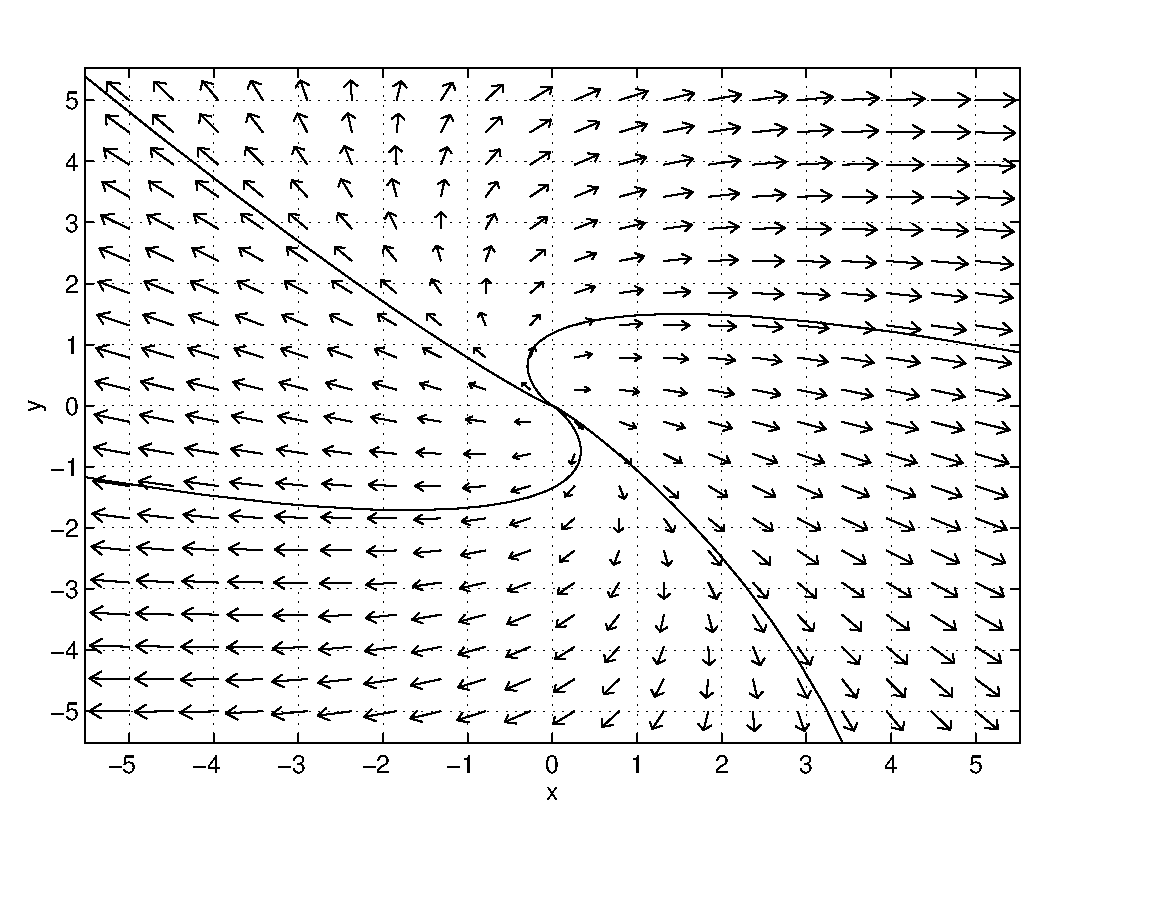
\psfig{file=exfigure/6-8-4a.eps,width=3.0in}}
		\exercap{c6.8.4a}
\end{figure}



\newpage
\subsection*{Section~\protect{\ref{S:6.9}} Phase Portraits of Nonhyperbolic
Systems}
\rhead{S:6.9}{PHASE PORTRAITS OF NONHYPERBOLIC SYSTEMS}

\exer{c6.9.1a} \ans One such matrix is $C = \mattwo{0}{-1}{1}{0}$.

\soln More generally, for any matrix
\[
C = \mattwo{\sigma}{-\tau}{\tau}{\sigma}
\]
such that $\sigma = 0$ and $\tau \neq 0$, the differential equation
$\dot{X} = CX$ will have the origin as a center.

\exer{c6.9.2}
Three trajectories of the undamped equation are shown in Figure~\ref{c6.9.2}a,
and one trajectory of the damped equation is shown in Figure~\ref{c6.9.2}b.

\begin{figure}[htb]
                       \centerline{%
                       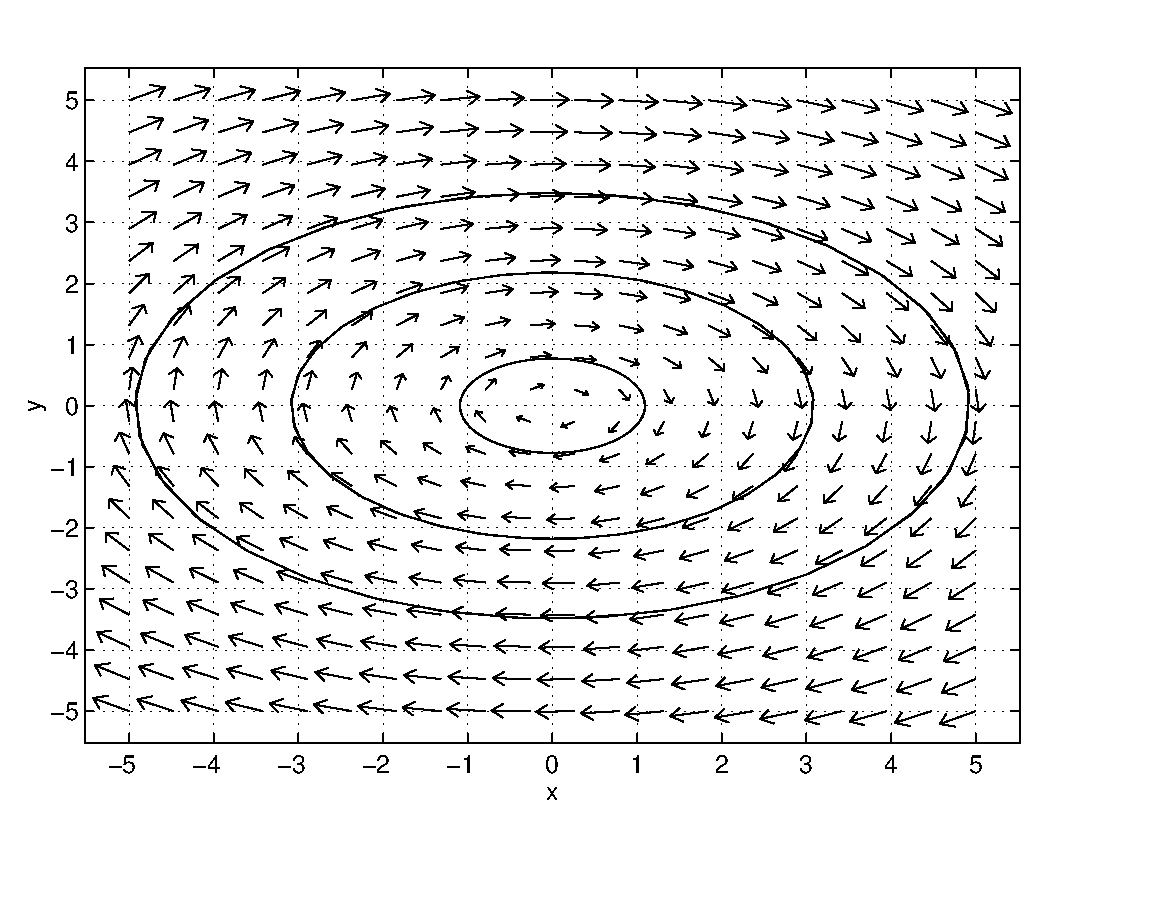
\psfig{file=exfigure/3-5-6a.eps,width=2.75in}
                       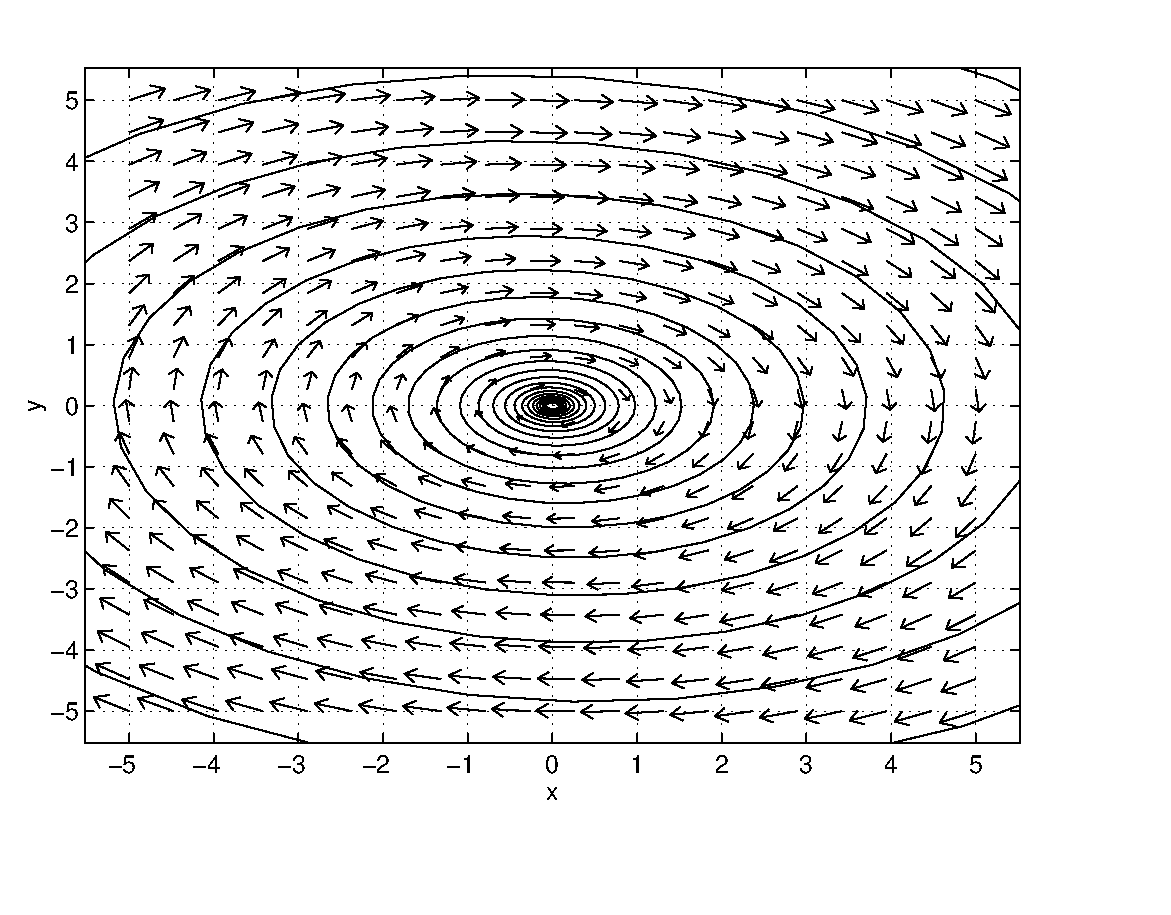
\psfig{file=exfigure/3-5-6b.eps,width=2.75in}}
			\exercaptwo{c6.9.2}
\end{figure}

\exer{E:PPb} \ans The origin is asymptotically stable for $A$ and unstable
for $B$, $C$ and $D$.

\soln The origin is asymptotically stable if all solutions tend towards
the origin as $t \rightarrow \infty$.

\exer{E:PPd} \ans The determinants of $A$ and $D$ are positive, the
determinant of $B$ is negative, and the determinant of $C$ is zero.

\soln The determinant of a matrix is the product of the eigenvectors.  The
eigenvectors of $A$ are complex conjugates, so their product
is positive.  A saddle has one negative and one positive eigenvector, so
the determinant of $B$ is negative.  A saddle node has one zero
eigenvector, so the product of the eigenvectors of $C$ is zero.  An
improper nodal source has equal positive eigenvectors, so the determinant
of $D$ is positive.

\newpage
\exer{E:PQa} \ans The origin is hyperbolic, and the equilibrium at the origin
is a spiral source.

\soln The trace and determinant of $C$ are both nonzero, so the origin
is hyperbolic.  Since $\det(C) = 3 > 0$ and $\trace(C) = 2 > 0$,
the equilibrium at the origin is a source.  Since the discriminant
$D \equiv \trace(C)^2 - 4\det(C) = -8 < 0$, the origin is a spiral.

\exer{E:PQc} \ans The origin is hyperbolic, and the equilibrium at the origin
is an improper nodal source.

\soln The trace and determinant of $C$ are both nonzero, so the origin
is hyperbolic.  Since $\det(C) = 4 > 0$ and $\trace(C) = 4 > 0$,
the equilibrium at the origin is a source.  Since the discriminant
$D \equiv \trace(C)^2 - 4\det(C) = 0$, the eigenvalues of $C$ are equal.
Since $C$ is not a multiple of $I_2$, $C$ has only one eigenvector, so
the origin is an improper node.

\exer{E:PQe} \ans The origin is not hyperbolic, and the equilibrium at
the origin is a center.

\soln Since $\det(C) = 4 > 0$ and $\trace(C) = 0$, the origin is not
hyperbolic and $C$ has purely imaginary eigenvalues.  Thus, the
equilibrium at the origin is a center.

\exer{E:PQg} \ans The origin is hyperbolic, and the equilibrium at the origin
is a saddle.

\soln The trace and determinant of $C$ are both nonzero, so the origin
is hyperbolic.  Since $\det(C) = -3 < 0$, the equilibrium at the origin 
is a saddle.

\exer{c6.9.5}
By definition, a system $\dot{X} = CX$ is a shear if the system has two
zero eigenvalues.  In this case, $\det(C) = 0$ and $\trace(C) = 0$, so
the eigenvalues are $\lambda_1 = \lambda_2 = 0$.  The phase portrait of
this system is shown in Figure~\ref{c6.9.5}a, and the phase portrait of
\Ref{e:00} is shown in Figure~\ref{c6.9.5}b.  In both phase portraits,
all trajectories are straight lines parallel to the eigenvector.  However,
in \ref{c6.9.5}b, the trajectories are parallel to the $x$-axis, whereas
in \ref{c6.9.5}a, they are not.

\begin{figure}[htb]
                       \centerline{%
                       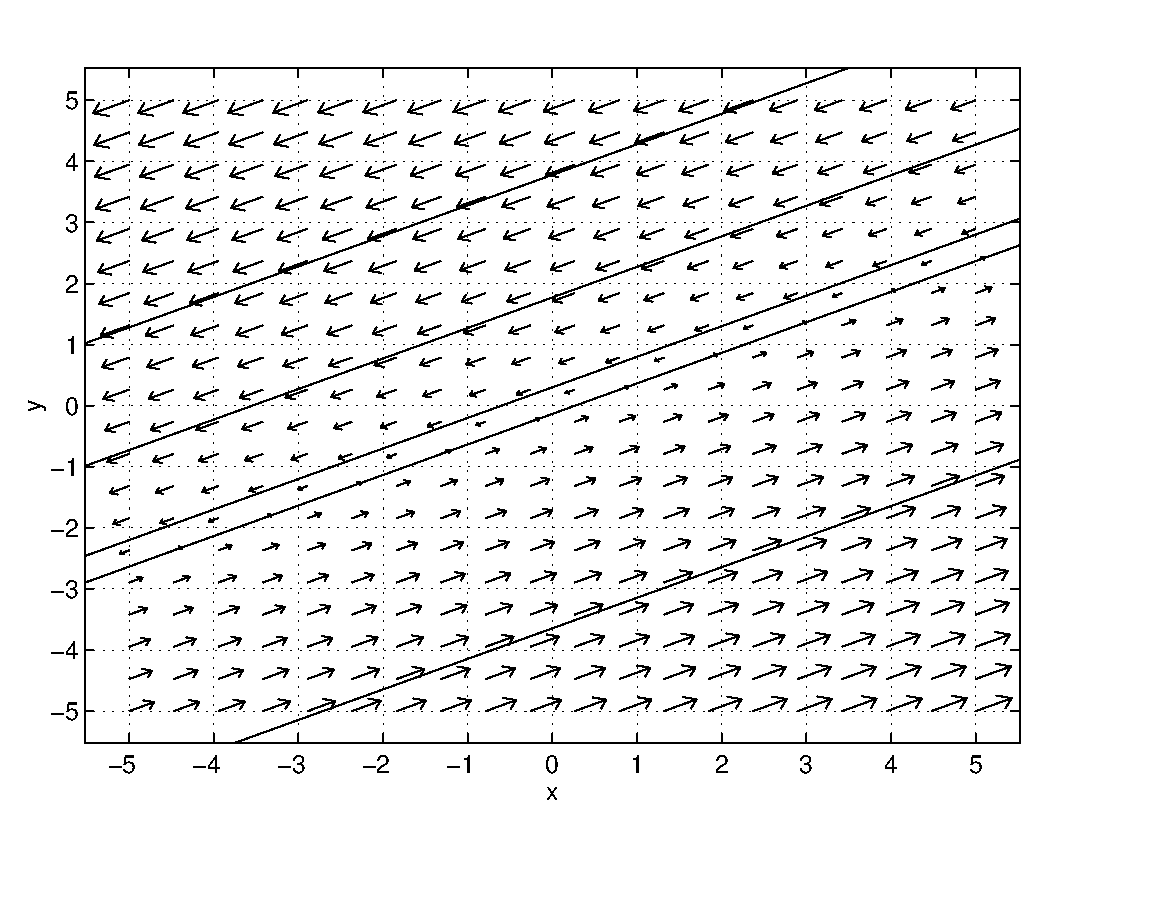
\psfig{file=exfigure/6-9-5a.eps,width=2.75in}
                       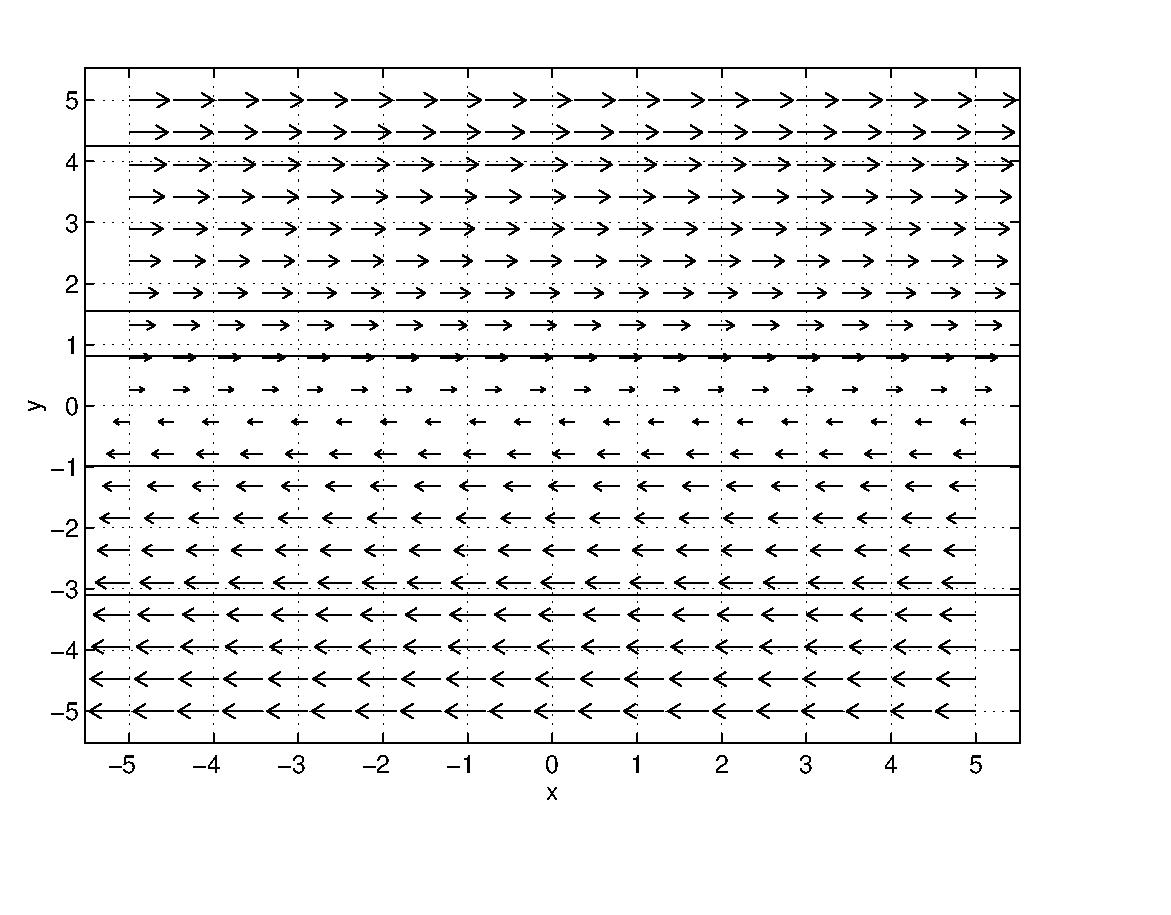
\psfig{file=exfigure/6-9-5b.eps,width=2.75in}}
                \exercaptwo{c6.9.5}
\end{figure}





\end{document}
